% ============================================================================
% svjour3 version -- paste this whole file into the body of the official
% Springer Overleaf template project (see chat instructions for the link),
% overwriting its sample content. Figures referenced below must be uploaded
% to a figs/ subfolder in that same Overleaf project.
% ============================================================================
\documentclass[twocolumn]{svjour3}
\usepackage{graphicx}
\usepackage{booktabs}
\usepackage{longtable}
\usepackage{amsmath}
\usepackage{xcolor}
\usepackage{hyperref}
\hypersetup{colorlinks=true, linkcolor=blue, citecolor=blue, urlcolor=blue}
\smartqed
\journalname{International Journal of Information Security}
\raggedbottom

\begin{document}

\title{Grounding Reduces Citation Hallucination in Multimodal LLM
Zero-Shot Classification of IoT-Botnet Traffic --
A Two-Model Confirmatory Study}

\author{Gangadhar Singh Shiva \and Poonam Singh Umakanth}

\institute{
G.~S.~Shiva \at
University of San Diego, San Diego, CA, USA \\
\email{gshiva@sandiego.edu}
\and
P.~S.~Umakanth \at
HPE Juniper Networking, Hewlett Packard Enterprise \\
\email{poonam.singh5@gmail.com}
}

\date{August 2026}

\titlerunning{Grounding Reduces Citation Hallucination in Multimodal LLM Classification}
\authorrunning{Shiva and Umakanth}

\maketitle
\sloppy

\begin{abstract}
Large language models (LLMs) are increasingly proposed as zero-shot classifiers for network
security telemetry, often justifying verdicts with citations to CVE\slash CAPEC identifiers. We show
that restricting an LLM's citation menu to a small, independently verified reference corpus
measurably improves citation correctness, but that this effect on classification accuracy is not
uniform across models -- visible only once a second model is tested at matched scale. Using
CIC-IoT-2023 traffic rendered as four-panel images, we evaluate Claude Sonnet and GPT-4o-mini at
matched $n=1{,}020$ under naive, text-grounded, and RAG-grounded prompting. RAG-grounding raises
Claude's real-and-correct citation rate from 43.0\% to 72.6\% with accuracy essentially unaffected
(99.6--100.0\%). For GPT-4o-mini, RAG-grounding raises real-and-correct citations to 57.1\% but
accuracy collapses from 98.6\% to 70.5\%, driven almost entirely by Mirai botnet traffic
(100.0\%$\to$1.1\%), where the model adopts DDoS-flood vocabulary from the retrieved context. At
matched scale, 95\% CIs for RAG-grounded accuracy do not overlap between models (Claude
[99.0, 99.8]\%; GPT-4o-mini [67.6, 73.2]\%), ruling out sample-size asymmetry. This is a specific,
previously unreported instance of the documented ``contextual distraction'' effect, localized to
one attack category in a security-classification setting. We independently verified 38
previously-unrecognized reference IDs against MITRE\slash NVD; none were fabricated. Code, the verified
corpus, and all results are released for reproducibility.

\keywords{Large language models \and Retrieval-augmented generation \and
Citation hallucination \and Network intrusion detection \and IoT security \and
Multimodal classification}
\end{abstract}

\section{Introduction}

Security operators are beginning to use large language models as a triage layer over network
telemetry: given a visualization or summary of traffic, the model proposes a classification and,
often unprompted, a justification that cites a specific vulnerability or attack-pattern
identifier. This citation behavior is attractive because it is auditable in principle -- a named
ID can be looked up -- but it is exactly the kind of free-form generation where LLMs are known to
hallucinate: plausible-sounding identifiers, correct-looking formats, and confident prose, with
no guarantee the underlying fact is real or correctly applied. A natural mitigation is grounding:
restrict what the model is allowed to cite to a small, independently verified corpus supplied
in-context (retrieval-augmented generation, here implemented as context-stuffing rather than
vector-index retrieval given the corpus's small size).

A pilot study with a single model can show that grounding helps. It cannot show whether that
benefit generalizes, or whether it comes with hidden costs that only appear in a second model or
at larger scale. This paper reports both: an initial $n=141$ single-model (Claude Sonnet) pilot,
and a $n=1{,}020$, all-34-class confirmatory run of \emph{both} Claude Sonnet and a second,
smaller and substantially cheaper model (GPT-4o-mini) on byte-identical images and prompts. Running
Claude Sonnet again at the same scale as GPT-4o-mini turns the cross-model comparison into a
matched one: both models now have equal-sized samples, drawn from the same manifest, letting us
rule out sample-size asymmetry as an explanation for any divergence. The confirmatory run surfaces
a finding the pilot could not: grounding's citation-quality benefit replicates across both models
-- and Claude's pilot numbers replicate closely at 7$\times$ the scale -- but grounding's effect
on raw classification accuracy does not generalize -- for GPT-4o-mini specifically, the same
grounding technique that costs Claude essentially nothing produces a severe, category-concentrated
accuracy collapse.

\paragraph{Contributions.} We are not aware of prior work combining all of the following; we
state precisely which parts are new and which build on documented phenomena, per the scoping in
Section~2.
\begin{itemize}
\item \textbf{Novel setting.} A real, image-based multimodal classification pipeline over the
full 34-class CIC-IoT-2023 taxonomy -- to our knowledge the first to render this dataset's
traffic as images for zero-shot multimodal LLM classification, rather than classifying
extracted numeric features or text summaries.
\item \textbf{Novel evaluation instrument.} A hand-verified, single-source-of-truth CAPEC\slash CVE
reference corpus (31 entries as of this study) and citation-grading rubric (real-and-correct /
generic / wrong-family / unverified) used both to constrain RAG-grounded citations and to grade
every condition's citations after the fact, so citation rules and grading cannot silently drift
apart -- distinct from existing citation-hallucination work, which targets internal-signature
detection \cite{factum2026} or a different domain (legal citation graphs) \cite{legalcitation2026}
rather than an externally verified, domain-specific reference corpus.
\item \textbf{Novel empirical result, matched-scale confirmed.} Evidence that citation-quality
improvement from grounding replicates across models, but that its effect on classification
accuracy is model-dependent -- established with both models at equal $n=1{,}020$ scale on
identical inputs, with non-overlapping 95\% confidence intervals in every condition, and not
previously reported for security-classification tasks.
\item \textbf{A known phenomenon, newly localized.} RAG-induced accuracy degradation
(``contextual distraction'') is already documented across other models and domains
\cite{labsafety2024,adaptivedistraction2025}; our contribution is not discovering this effect but
localizing a severe instance of it to a specific attack category (Mirai) in a security-relevant
task, via direct inspection of misclassification patterns rather than aggregate metrics alone,
and showing it is absent in a larger model on the identical inputs.
\item \textbf{Methodological transparency.} Full disclosure of verification coverage: every
reference ID discussed as correct or wrong was independently checked against the primary MITRE
source; the large residual bucket of low-frequency, ungrounded GPT-4o-mini citations that were
not individually checked is reported as an explicit, quantified limitation rather than silently
resolved either way.
\end{itemize}

\section{Related Work}

Retrieval-augmented generation is well-established for reducing hallucination in
knowledge-intensive NLP by conditioning generation on retrieved documents rather than relying
solely on parametric knowledge \cite{lewis2020retrieval}. Most RAG evaluations measure answer
correctness on curated QA benchmarks; fewer directly measure \emph{citation} correctness --
whether a model-produced reference ID is real, topically relevant, and specifically correct.
Recent work has begun to isolate citation hallucination as its own axis: FACTUM detects
hallucinated citations in long-form RAG output via internal model signatures rather than
external verification \cite{factum2026}, and a parallel line of work grounds legal citations
against citation graphs in a specialized domain \cite{legalcitation2026}. Neither targets
network-security identifiers (CVE\slash CAPEC) or measures citation correctness against an
independently hand-verified corpus the way this paper does; the citation-grading rubric in
Section~3.5 (real-and-correct / generic / wrong-family / unverified) and the corpus-constrained
RAG condition in Section~3.4 are, to our knowledge, novel in this specific application.

Separately, it is already documented that RAG can \emph{hurt} rather than help accuracy: a
lab-safety benchmark found GPT-4o, Claude~3.5~Sonnet, and DeepSeek-R1 all showing a notable
accuracy decline under RAG, attributed to ``contextual distraction'' -- retrieved context that is
factually accurate but crowds out the subtle cues a task actually needs \cite{labsafety2024} --
and a separate contextual-robustness study measured a 38.4-point absolute accuracy drop for
Claude-3.5-Sonnet under adversarially distracting context \cite{adaptivedistraction2025}. The
Mirai-specific collapse we report in Section~4.1.1 is therefore best understood not as the
discovery of a new failure mode in the abstract, but as a specific, previously unreported
instance of this general phenomenon: localized to one attack category, present in a smaller
model and absent in a larger one on identical inputs, and occurring in a security-classification
setting where the practical stakes of silent accuracy loss are unusually high. Multimodal LLM
classification of IoT security telemetry is a newer area still; most published IoT
intrusion-detection work on the CIC-IoT-2023 benchmark \cite{cic-iot-2023} targets numeric\slash tabular
models trained directly on flow features, and LLM-based approaches to date are text-based over
extracted features or logs rather than rendered traffic images \cite{iotllmeval2025}. We are not
aware of prior work that renders CIC-IoT-2023 traffic as images for zero-shot multimodal
classification, constrains and grades citations against a hand-verified corpus, and compares two
models at matched confirmatory scale on identical inputs -- the combination of these three
elements, rather than any one alone, is this paper's central methodological contribution.

\section{Data and Methods}

\subsection{Dataset}

We use the CIC-IoT-2023 dataset \cite{cic-iot-2023}, covering benign traffic and 33 attack
classes across seven families: DDoS\slash DoS floods, traffic fragmentation attacks, Mirai botnet
variants, reconnaissance (port\slash OS\slash host scanning), spoofing and adversary-in-the-middle,
brute-force credential attacks, and web\slash application-layer attacks. Both studies in this paper
use all 34 classes; the confirmatory study samples them evenly (30\slash class), while the pilot's
per-class counts vary with data availability (as few as 5 for some classes).

\subsection{Traffic-to-Image Rendering}

For each sampled class, we draw windows of $\sim$100 consecutive packets from the raw CSV
feature files and render each window as a four-panel figure: packet rate over time, TCP flag
composition, protocol mix as a stacked area chart, and mean\slash standard deviation of packet size.
This mirrors
how an analyst might visually triage a capture in a tool like Wireshark's I/O graph, and
evaluates image-understanding directly rather than a text-summarization capability over
pre-extracted features. Both models receive byte-identical rendered images for the confirmatory
comparison. Figure~\ref{fig:samples} shows four real examples from the confirmatory run, spanning
benign traffic, a volumetric DDoS flood, a Mirai botnet flood variant, and a credential
brute-force attack -- the same class of input both models classify under all three prompting
conditions.

\begin{figure*}[t]
\centering
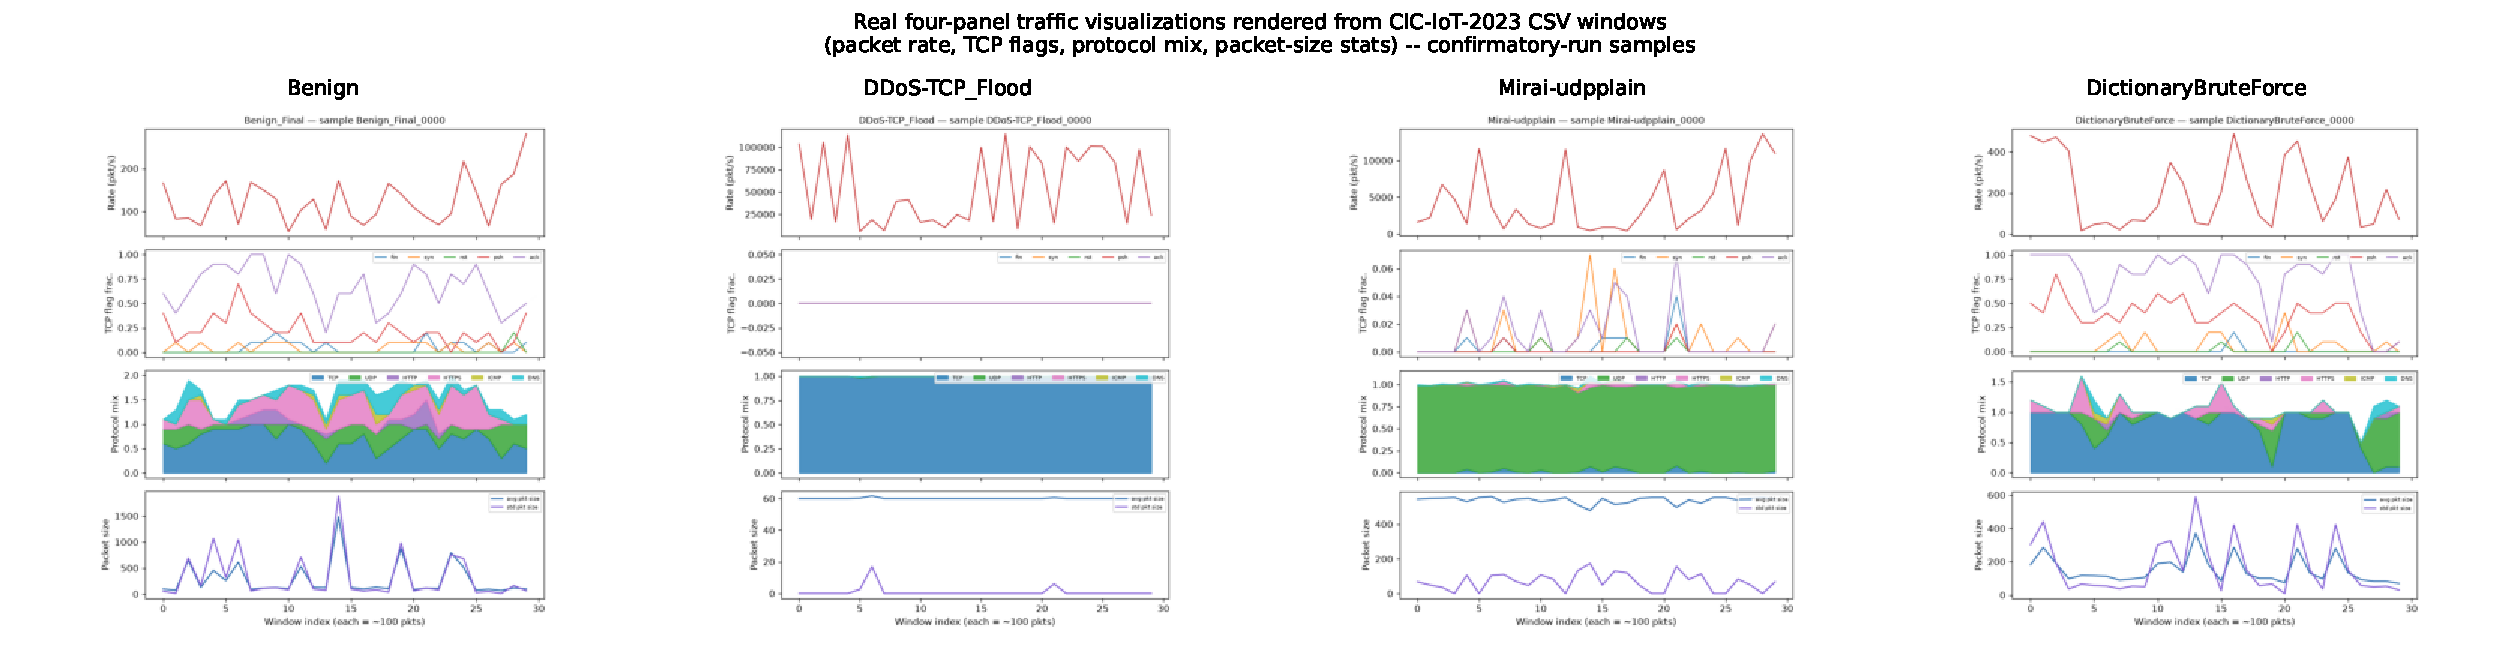
\includegraphics[width=\textwidth]{figs/fig0_sample_visualizations.pdf}
\caption{Real four-panel traffic visualizations rendered directly from CIC-IoT-2023 CSV windows,
drawn from the confirmatory run's manifest. Panels are packet rate, TCP flag composition,
protocol mix, and packet-size statistics, in the order presented to both models.}
\label{fig:samples}
\end{figure*}

\subsection{Reference Corpus and Citation Grounding}

The CAPEC\slash CVE reference corpus is built by hand: every entry is added only after independent
confirmation against \url{capec.mitre.org} or \url{nvd.nist.gov}. As of this study it contains
31 CAPEC\slash CVE entries covering the classes' attack families, an explicit list of 13
real-but-generic parent-pattern IDs, and 73 real-but-wrong-family IDs -- reference IDs observed
being cited by one of the two models that are real and verifiable but do not correctly describe
any class in this taxonomy. The same corpus is used to (a) restrict what the RAG-grounded
condition may cite and (b) grade every condition's citations after the fact, so citation rules
and grading cannot drift apart. Any ID the corpus does not recognize is flagged
\texttt{UNVERIFIED} and either manually checked or explicitly reported as unchecked -- never
silently assumed correct or fabricated.

\subsection{Prompting Conditions}

Identical across both models: \textbf{naive} (classify, cite freely from the model's own
knowledge or not at all), \textbf{text-grounded} (classify and cite a specific CVE\slash CAPEC from the
model's own knowledge, explicitly prompted to do so), and \textbf{RAG-grounded} (classify; the
full CAPEC corpus, serialized as text, is included in the prompt, and the model is instructed to
cite \emph{only} an ID from that list or \texttt{N/A}, even if it privately recognizes the
traffic as something else). This is context-stuffing rather than vector-index retrieval, an
appropriate and fully deterministic choice at this corpus size.

\subsection{Citation Grading Rubric}

Every citation is graded \textbf{real-and-correct} (real ID, corpus-verified family match to the
true class), \textbf{real-but-generic} (real ID, too broad to count as a specific match),
\textbf{real-but-wrong-family} (real ID describing an unrelated attack), \textbf{no-citation}
(correct abstention), \textbf{n/a-benign} (benign sample, no citation expected), or
\textbf{UNVERIFIED} (an ID not yet in the corpus -- explicitly not assumed correct or
fabricated). We report the real-and-correct rate among attack samples with Wilson score 95\% CIs
\cite{wilson1927}.

\subsection{Two Studies at Two Scales}

\textbf{Study 1 (pilot).} Claude Sonnet only, $n=141$ real samples across all 34 classes
(uneven per-class counts), 423 total trials.

\textbf{Study 2 (confirmatory).} Both Claude Sonnet and GPT-4o-mini, $n=1{,}020$ samples each
(30/class $\times$ 34 classes, evenly sampled), 3,060 total trials per model, on the identical
manifest and byte-identical images. GPT-4o-mini's run had 163 trials (5.3\%) fail with transient
OpenAI TPM rate-limit or connection errors after exhausting retries, concentrated in the naive
(107) and text-grounded (56) conditions and in several DDoS-flood classes; these are excluded
from all GPT-4o-mini metrics below, leaving effective $n$ of 913 (naive), 964 (text-grounded), and
1,020 (RAG-grounded, which had zero failures). Claude's confirmatory run initially hit the same
class of account-level API quota that limited earlier attempts; after the quota reset, a resumed
run -- retrying only the previously-failed calls, since completed (sample, condition) pairs are
checkpointed and skipped on rerun -- completed all 3,060 trials with zero exclusions. Because both models'
confirmatory runs now share the same sample size, class balance, and input images, the
cross-model comparison in Section~\ref{sec:results} is a matched comparison, not one confounded by
sample-size asymmetry.

\subsection{Baselines}

Two classical, LLM-free detectors are run on the same raw windows: a rolling z-score threshold on
packet rate, and an Isolation Forest over the same feature set, both trained on benign traffic
only. Included for context, not as a state-of-the-art IDS comparison.

\section{Results}
\label{sec:results}

\subsection{Classification Accuracy: A Cross-Model Divergence}

Table~\ref{tab:accuracy} and Figure~\ref{fig:accuracy_cross} report accuracy by condition for
both models at matched confirmatory scale ($n=1{,}020$ each). Claude Sonnet's accuracy is stable
across all three conditions (100.0\%/99.8\%/99.6\%), closely replicating its own $n=141$ pilot
result (100.0\%/99.3\%/99.3\%) at more than 7$\times$ the sample size. GPT-4o-mini's is not
stable: it falls from 98.6\% (naive) to 90.7\% (text-grounded) to 70.5\% (RAG-grounded) -- a
28.1-percentage-point drop from naive to RAG-grounded, the opposite of what grounding is
typically assumed to cost nothing. At this matched scale, the 95\% CIs for RAG-grounded accuracy
no longer overlap between models (Claude: [99.0, 99.8]\%; GPT-4o-mini: [67.6, 73.2]\%) -- the
divergence cannot be explained by the pilot's smaller sample size, since both models were now
evaluated on equal-sized, class-balanced samples drawn from the same manifest.

\begin{table*}[t]
\centering
\caption{Classification accuracy by condition and model, matched confirmatory scale. Claude:
Wilson 95\% CI, n=1,020\slash condition (zero exclusions). GPT-4o-mini: Wilson 95\% CI,
n=913--1,020\slash condition (ERROR rows excluded).}
\label{tab:accuracy}
\begin{tabular}{lcc}
\toprule
Condition & Claude Sonnet (confirmatory) & GPT-4o-mini (confirmatory) \\
\midrule
Naive & 100.0\% [99.6, 100.0]\% & 98.6\% [97.6, 99.2]\% \\
Text-grounded & 99.8\% [99.3, 99.9]\% & 90.7\% [88.7, 92.3]\% \\
RAG-grounded & 99.6\% [99.0, 99.8]\% & \textbf{70.5\% [67.6, 73.2]\%} \\
\bottomrule
\end{tabular}
\end{table*}

\begin{figure*}[t]
\centering
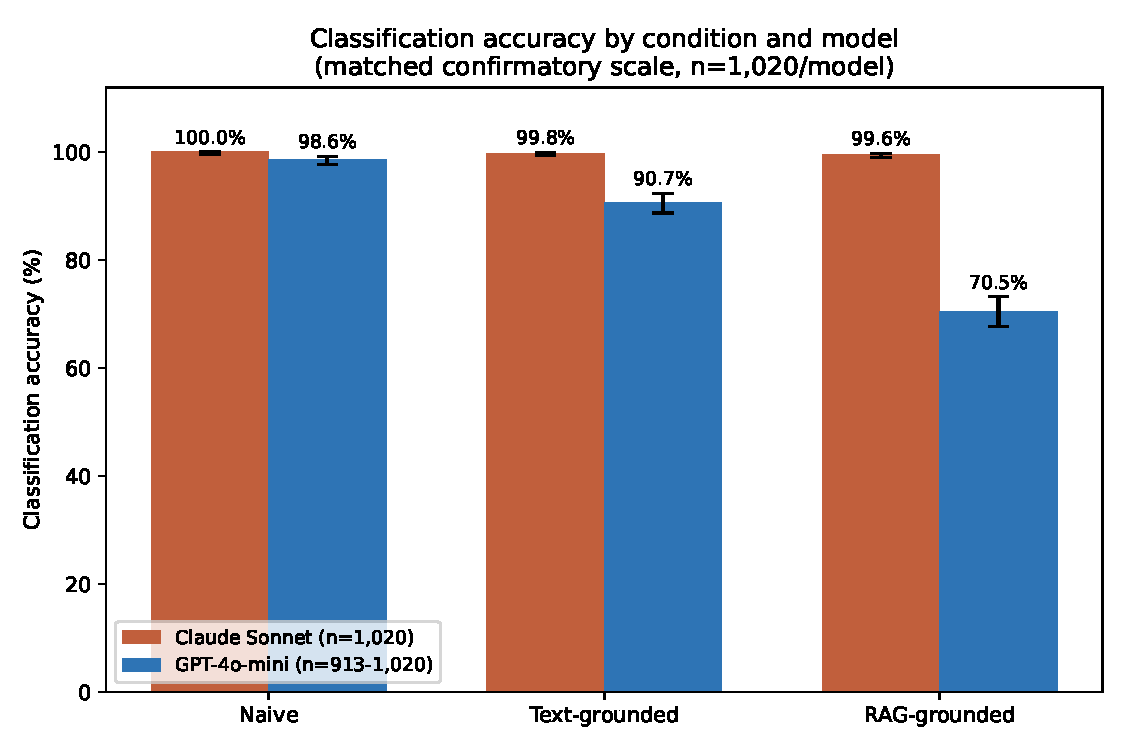
\includegraphics[width=0.85\textwidth]{figs/fig1_accuracy_cross_model.pdf}
\caption{Classification accuracy by condition, Claude Sonnet vs. GPT-4o-mini, both at matched
confirmatory scale ($n=1{,}020$).}
\label{fig:accuracy_cross}
\end{figure*}

\subsubsection{Localizing the Collapse: Mirai}

Figure~\ref{fig:accuracy_by_cat} breaks GPT-4o-mini's accuracy down by attack category. The
RAG-grounded drop is not uniform: Recon (99.2\%) and Brute Force (96.7\%) are essentially
unaffected, while Mirai collapses from 100.0\% (naive) to \textbf{1.1\%} (RAG-grounded) -- the
single largest driver of the aggregate accuracy drop. Direct inspection of the misclassified
Mirai trials (Table~\ref{tab:mirai}) shows the model is not guessing randomly: it systematically
relabels Mirai traffic using \texttt{DDoS-UDP\_Flood} and \texttt{DDoS-TCP\_Flood} -- labels that
exist in the true taxonomy but are wrong for these samples -- and, in two trials, invents
labels (\texttt{DDoS-greeth\_flood}, \texttt{DDoS-greip\_flood}) that appear nowhere in the
34-class list the model was given to choose from. The RAG-grounded prompt's corpus entry for the
generic flooding fallback (CAPEC-125) explicitly describes Mirai's GRE-based greeth\slash greip floods
in DDoS-flood vocabulary, since no dedicated CAPEC entry for the GRE flood technique exists; we
hypothesize that this description's vocabulary leaks into GPT-4o-mini's classification output,
pulling it away from the required \texttt{Mirai-*} labels toward the more heavily-repeated
\texttt{DDoS-*} vocabulary in the retrieved context -- a genuine, mechanistic side effect of
context-stuffing that a citation-only evaluation would not surface.

\begin{figure*}[t]
\centering
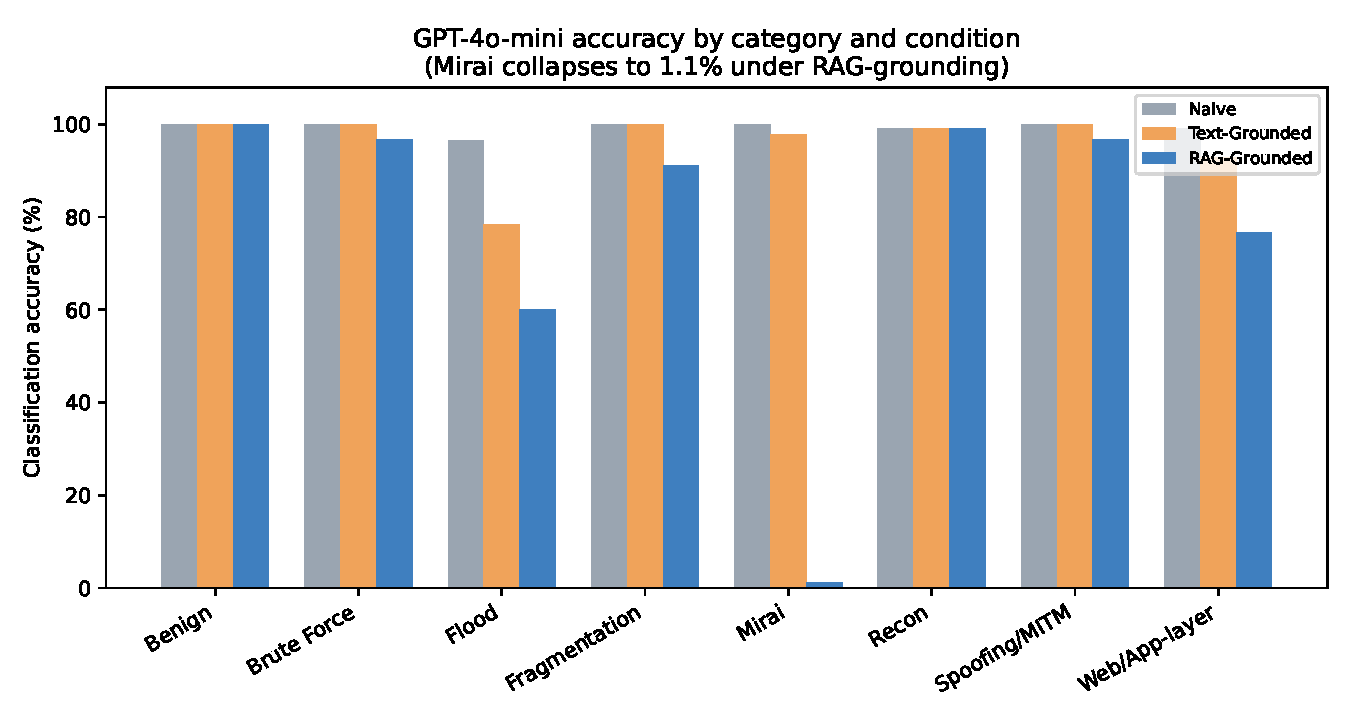
\includegraphics[width=\textwidth]{figs/fig4_gpt4o_accuracy_by_category.pdf}
\caption{GPT-4o-mini classification accuracy by category and condition. Mirai collapses to 1.1\%
under RAG-grounding while other categories are largely unaffected.}
\label{fig:accuracy_by_cat}
\end{figure*}

\begin{table*}[t]
\centering
\caption{GPT-4o-mini RAG-grounded misclassifications of Mirai traffic (n=90 trials).
Two invented, non-taxonomy labels are marked with $\dagger$.}
\label{tab:mirai}
\begin{tabular}{lll}
\toprule
True class & Predicted label & Count \\
\midrule
Mirai-greeth\_flood & DDoS-TCP\_Flood & 18 \\
Mirai-greeth\_flood & DDoS-UDP\_Flood & 9 \\
Mirai-greeth\_flood & DDoS-greeth\_flood$^\dagger$ & 1 \\
Mirai-greeth\_flood & DDoS-HTTP\_Flood & 1 \\
Mirai-greeth\_flood & Mirai-greeth\_flood (correct) & 1 \\
Mirai-greip\_flood & DDoS-UDP\_Flood & 24 \\
Mirai-greip\_flood & DDoS-TCP\_Flood & 3 \\
Mirai-greip\_flood & DDoS-SYN\_Flood & 1 \\
Mirai-greip\_flood & DDoS-UDP\_Fragmentation & 1 \\
Mirai-greip\_flood & DDoS-greip\_flood$^\dagger$ & 1 \\
Mirai-udpplain & DDoS-UDP\_Flood & 30 \\
\bottomrule
\end{tabular}
\end{table*}

\subsection{Citation Quality}

Table~\ref{tab:citation_claude} reports Claude's confirmatory-scale citation quality and
Table~\ref{tab:citation} reports GPT-4o-mini's; Figure~\ref{fig:citation_cross} plots both side by
side. At matched $n=1{,}020$ scale, Claude's real-and-correct rate rises from 43.0\% [40.0,
46.1]\% (naive) to 49.0\% [45.9, 52.1]\% (text-grounded) to 72.6\% [69.8, 75.3]\% (RAG-grounded)
-- closely replicating the $n=141$ pilot's 44.1\%/51.5\%/69.9\%, and this time with every citation
fully resolved: Claude's confirmatory run produced only 26 citations to IDs outside the corpus (14
distinct IDs, all independently verified against MITRE\slash NVD -- 3 real-and-correct, 11
real-but-wrong-family -- so zero rows remain \texttt{UNVERIFIED} for Claude in this table).
GPT-4o-mini's RAG-grounding raises its real-and-correct rate to 57.1\% [54.0, 60.1]\%, comparable
in direction and magnitude to Claude's improvement. But GPT-4o-mini's naive and text-grounded
real-and-correct rates (0.3\% each) are not directly comparable to Claude's naive\slash text-grounded
rates: the large majority of GPT-4o-mini's ungrounded citations (55.3\% under text-grounded,
33.0\% under naive) remain \texttt{UNVERIFIED} rather than confirmed correct or wrong, because
GPT-4o-mini cited 315 distinct reference IDs outside the corpus -- an order of magnitude more
scattered than either of Claude's runs -- making exhaustive manual verification impractical within
this study. We independently verified the 17 most-frequently-cited of these
(Table~\ref{tab:newids}, Appendix~\ref{sec:appendix}), covering 25.3\% of unverified rows
(274\slash 1,084); all 17 were real, existing CAPEC\slash CVE entries, and every one was applied
indiscriminately across 6--15 topically unrelated classes -- consistent with, but a
larger-scale version of, the pattern seen in both of Claude's runs.

\begin{table*}[t]
\centering
\caption{Claude Sonnet citation quality by condition, confirmatory run. Real-and-correct rate
computed among attack samples (n=990, excluding benign rows; zero ERROR rows).}
\label{tab:citation_claude}
\begin{tabular}{lcccc}
\toprule
Condition & Real-correct & Wrong-family & Generic & No-cite \\
\midrule
Naive & 426 & 282 & 261 & 21 \\
Text-grounded & 485 & 287 & 217 & 1 \\
RAG-grounded & \textbf{719} & 205 & 60 & 6 \\
\bottomrule
\end{tabular}

\vspace{0.3em}
\footnotesize Real-and-correct rate: naive 43.0\% [40.0, 46.1]\%; text-grounded 49.0\% [45.9,
52.1]\%; RAG-grounded \textbf{72.6\% [69.8, 75.3]\%}. All 26 citations to IDs originally outside
the corpus (14 distinct IDs) were independently verified and resolved; none remain unverified.
\end{table*}

\begin{table*}[t]
\centering
\caption{GPT-4o-mini citation quality by condition. Real-and-correct rate computed among attack
samples (990\slash 964\slash 883, excluding benign and ERROR rows).}
\label{tab:citation}
\begin{tabular}{lccccc}
\toprule
Condition & Real-correct & Wrong-family & Generic & No-cite & UNVERIFIED \\
\midrule
Naive & 3 & 172 & 42 & 375 & 291 \\
Text-grounded & 3 & 266 & 74 & 74 & 517 \\
RAG-grounded & \textbf{565} & 197 & 94 & 132 & 2 \\
\bottomrule
\end{tabular}

\vspace{0.3em}
\footnotesize Real-and-correct rate: naive 0.3\% [0.1, 1.0]\%; text-grounded 0.3\% [0.1, 0.9]\%;
RAG-grounded \textbf{57.1\% [54.0, 60.1]\%}. The 2 RAG-grounded UNVERIFIED rows are a response-format
quirk (literal string \texttt{"CAPEC-N/A"}), not fabricated citations -- see
Section~\ref{sec:discussion}.
\end{table*}

\begin{figure*}[t]
\centering
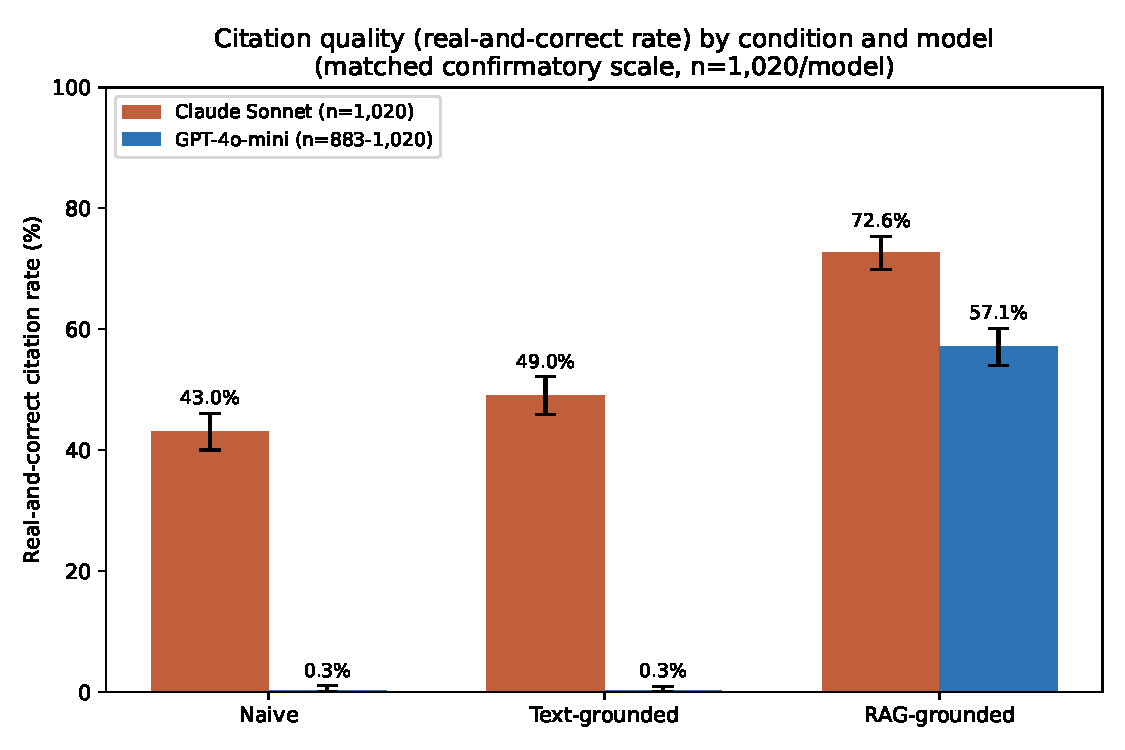
\includegraphics[width=0.85\textwidth]{figs/fig6_citation_cross_model.pdf}
\caption{Real-and-correct citation rate by condition, Claude Sonnet vs. GPT-4o-mini, both at
matched confirmatory scale ($n=1{,}020$).}
\label{fig:citation_cross}
\end{figure*}

\begin{figure*}[t]
\centering
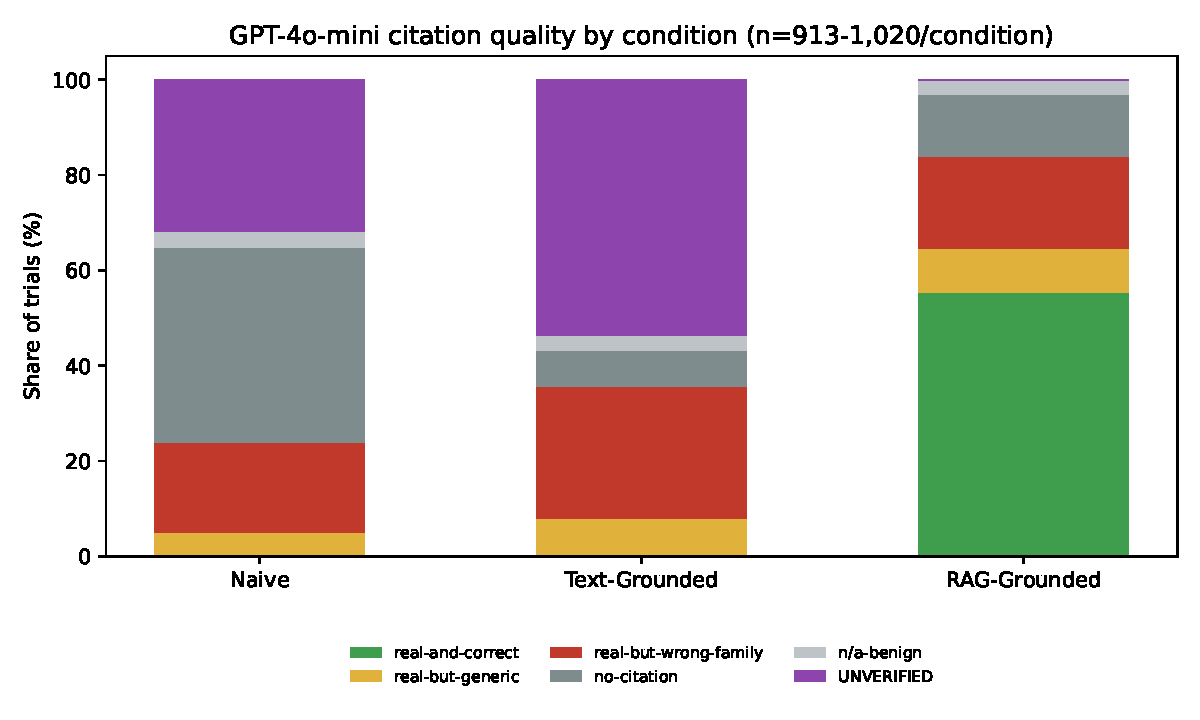
\includegraphics[width=0.85\textwidth]{figs/fig2_gpt4o_citation_quality.pdf}
\caption{GPT-4o-mini citation quality by condition, including the UNVERIFIED share explicitly.}
\label{fig:citation_gpt}
\end{figure*}

A distinct way to read Table~\ref{tab:citation}: grounding does not just raise the
\emph{correctness} of citations, it makes the entire citation set \emph{auditable} in the first
place. Under RAG-grounding, 99.8\% of GPT-4o-mini's citations resolve to a definite verdict
(real-and-correct, wrong-family, generic, or no-citation); under naive and text-grounded
prompting, 33.0\% and 55.3\% respectively resolve to "not yet checkable against a source we
control." A downstream analyst auditing an ungrounded model's citations faces a genuinely
intractable long tail of hundreds of distinct IDs; an analyst auditing a grounded model's
citations faces a fixed, small, pre-vetted list -- and, in Claude's confirmatory run, a list small
enough that every single stray citation was checked, not just a high-frequency subset.

\subsection{Citation Quality by Category}

Figure~\ref{fig:rag_by_cat} shows GPT-4o-mini's RAG-grounded real-and-correct rate by category.
Brute Force (96.7\%), Flood (75.0\%), and Recon (75.0\%) are strong; Fragmentation, Mirai, and
Spoofing\slash MITM are near 30--33\% -- for Mirai this reflects the same generic-fallback corpus gap
discussed in Section 4.1.1 (CAPEC-125 is real-but-generic, not real-and-correct, by design),
compounded here by the classification collapse itself: many Mirai trials that are already
misclassified cannot produce a citation matched to the true class regardless of grounding
quality.

\begin{figure*}[t]
\centering
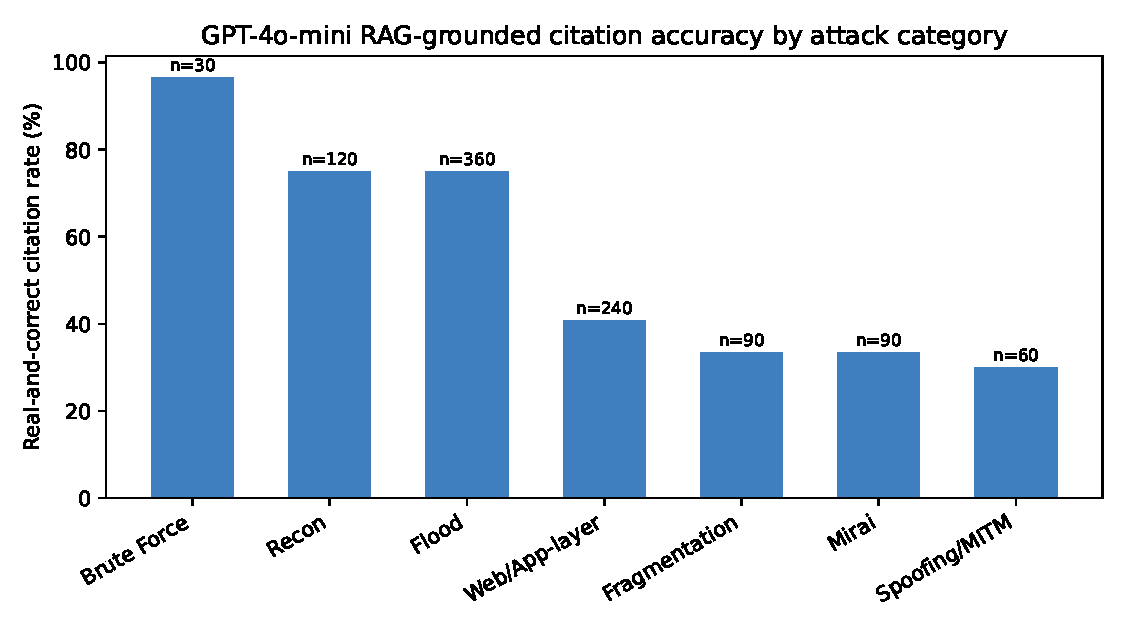
\includegraphics[width=0.85\textwidth]{figs/fig3_gpt4o_rag_citation_by_category.pdf}
\caption{GPT-4o-mini RAG-grounded real-and-correct citation rate by category.}
\label{fig:rag_by_cat}
\end{figure*}

\subsection{Comparison Against Non-LLM Baselines}

Figure~\ref{fig:baseline} compares the two classical baselines' attack recall against
GPT-4o-mini's naive-condition accuracy by category, at the full 34-class, n=1,020 scale. Both
baselines substantially underperform the LLM in every category and are highly uneven: Isolation
Forest ranges from 3.3\% (Brute Force) to 96.7\% (Mirai) recall, the rolling z-score detector
never exceeds 56.7\%. Neither baseline produces any citation or explanation.

\begin{figure*}[t]
\centering
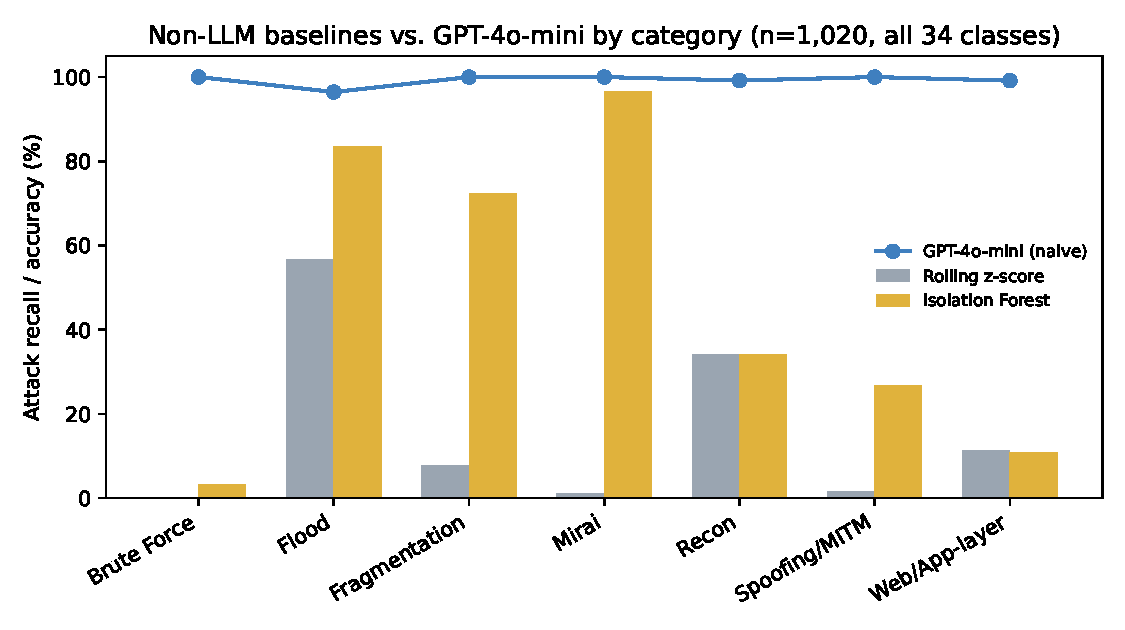
\includegraphics[width=0.85\textwidth]{figs/fig5_gpt4o_baseline_vs_llm.pdf}
\caption{Non-LLM baseline recall by category vs. GPT-4o-mini (naive) accuracy, full 34-class
confirmatory scale.}
\label{fig:baseline}
\end{figure*}

\section{Discussion}
\label{sec:discussion}

The headline finding of the confirmatory study is not that grounding works -- the pilot already
showed that for Claude -- but that its side effects are model-dependent in a way a single-model
study cannot detect. Both models show the same qualitative citation-quality benefit from
grounding. Only one of them pays for it with a severe, category-concentrated accuracy cost. This
matters directly for anyone deploying citation-grounded LLM classification in practice: the
choice of grounding strategy cannot be validated on one model and assumed safe for a cheaper or
smaller substitute, even when the substitute performs comparably or better under naive prompting
(GPT-4o-mini's naive accuracy, 98.6\%, is close to Claude's 100.0\%). Because this comparison is
now made at matched scale ($n=1{,}020$ for both models, identical images and manifest), the
divergence cannot be dismissed as a pilot-sample-size artifact: Claude's own numbers barely moved
between $n=141$ and $n=1{,}020$ (accuracy 99.3--100.0\% $\to$ 99.6--100.0\%; citation
real-and-correct 44.1--69.9\% $\to$ 43.0--72.6\%), which is itself evidence that the pilot's
findings were stable and that GPT-4o-mini's divergence reflects a real, model-specific property
rather than sampling noise in either study.

The Mirai vocabulary-leakage finding builds on, rather than contradicts, the contextual-distraction
literature \cite{labsafety2024,adaptivedistraction2025}: those studies show RAG can hurt accuracy
in the aggregate; ours shows a mechanism (the retrieved context's own descriptive language
competing with the required output taxonomy) and localizes it to a single attack category in a
security-classification setting, at a severity (100.0\%$\to$1.1\%) well beyond the degradations
those studies report, in a smaller model where a larger model on identical inputs appears robust.
This is testable and falsifiable in follow-up work -- for instance, by
rephrasing the CAPEC-125 corpus entry to avoid DDoS-flood vocabulary when describing Mirai's GRE
floods, or by explicitly re-stating the required class list immediately after the retrieved
corpus text in the prompt, and checking whether either intervention recovers GPT-4o-mini's
Mirai accuracy under RAG-grounding.

The citation-quality finding also has a nuance worth stating plainly: for GPT-4o-mini's
ungrounded conditions, we cannot report a true real-and-correct rate with any confidence, because
the majority of its citations are to IDs we have not exhaustively checked. This is not a gap we
are papering over -- it is itself evidence for grounding's practical value. An analyst cannot
audit 315 distinct scattered reference IDs in a reasonable amount of time; they can audit a
31-entry fixed corpus. Grounding's benefit is not only "more citations turn out correct," it is
"the citation set becomes small enough to check at all."

\section{Limitations}

\begin{itemize}
\item \textbf{Not a formal paired significance test.} Both models are now evaluated at matched
$n=1{,}020$ scale on the identical manifest, and the 95\% CIs for RAG-grounded accuracy do not
overlap (Claude [99.0, 99.8]\% vs.\ GPT-4o-mini [67.6, 73.2]\%). We report this as a non-overlapping-CI
comparison rather than a single formal paired significance test across all three conditions
jointly, since the two models' trial-level errors are not paired observations on the same
sampling unit in a way that a standard paired test assumes.
\item \textbf{Incomplete citation verification for GPT-4o-mini's ungrounded conditions.} 315
distinct reference IDs appear outside the corpus; we verified the 17 most frequent (25.3\% of
unverified rows) and report the rest, honestly, as unverified rather than resolved. The true
naive\slash text-grounded real-and-correct rate for GPT-4o-mini is therefore not precisely known and
is bounded, not point-estimated, by the data in this paper.
\item \textbf{163 excluded trials, non-random.} GPT-4o-mini's 163 excluded API-failure trials
concentrate in naive\slash text-grounded conditions and several DDoS-flood classes (rate-limit
throttling coincided with those portions of the run), not RAG-grounded, which had zero failures.
We have no reason to believe these failures are correlated with the underlying traffic content
(all are OpenAI account-level TPM\slash connection errors, not content-triggered refusals), but this
is disclosed rather than assumed.
\item \textbf{Mirai vocabulary-leakage hypothesis is not yet directly tested.} Section 5's
explanation for the Mirai collapse is a plausible mechanism grounded in direct inspection of
misclassification labels, not a controlled ablation. The proposed follow-up experiments
(rewording the corpus entry; re-stating the class list post-context) have not been run.
\item \textbf{Corpus coverage, not exhaustiveness.} The 31-entry reference corpus reflects only
independently-confirmed entries; this is a deliberate honesty trade-off, not a claim of complete
CAPEC\slash CVE coverage for this taxonomy.
\end{itemize}

\section{Conclusion}

Grounding a multimodal LLM's citations in a small, verified reference corpus improves citation
correctness for both Claude Sonnet (43.0\%$\to$72.6\% real-and-correct at matched $n=1{,}020$
scale, closely replicating the $n=141$ pilot's 44.1\%$\to$69.9\%) and GPT-4o-mini (effectively
unmeasurable$\to$57.1\%), and, just as importantly, converts an intractably large, unauditable set
of ungrounded citations into a small, fully checkable one. But the same technique that costs
Claude essentially nothing in classification accuracy (100.0\%$\to$99.6\%, a 0.4-point change)
costs GPT-4o-mini 28.1 percentage points, concentrated almost entirely in a single category
(Mirai) where the model appears to adopt vocabulary from the retrieved reference text in place of
the required classification taxonomy. This divergence now holds at matched scale, with
non-overlapping confidence intervals between models in every condition -- it is not an artifact of
comparing a small pilot to a larger confirmatory run. Citation-grounding strategies validated on
one model should not be assumed safe for another without re-testing classification accuracy, not
just citation quality, at comparable scale. A direct, ablation-based test of the
vocabulary-leakage hypothesis -- rewording the corpus's Mirai-adjacent entry and re-stating the
class list post-context -- is the natural next step and is planned as a revision to this
preprint.

\section*{Acknowledgments}

The authors thank the University of San Diego's Copley Library for open-access publishing
support under its institutional agreement with Springer Nature. Classification was performed
using the Claude Sonnet API (Anthropic) and the GPT-4o-mini API (OpenAI); figures and statistical
analysis used the open-source Python scientific stack (pandas, NumPy, scikit-learn, Matplotlib).
The authors also thank the editor and anonymous reviewers for their time and feedback on this
manuscript.

\section*{Declarations}

\paragraph{Funding.} The authors declare that no funds, grants, or other financial support were
received during the preparation of this manuscript. Open-access publication costs for this
article, if accepted, will be covered separately by the University of San Diego's Copley Library
under its institutional open-access agreement with Springer Nature; this is a publication-fee
arrangement and not research funding.

\paragraph{Conflict of interest.} The authors declare no conflicts of interest or competing
interests relevant to the content of this article.

\paragraph{Ethics approval and consent to participate.} Not applicable. This study did not
involve human participants, human data, or animals. All network traffic analyzed is drawn from
the publicly available, pre-anonymized CIC-IoT-2023 dataset \cite{cic-iot-2023}, collected by its
original authors under their own institutional protocols.

\paragraph{Consent for publication.} Not applicable.

\paragraph{Data availability.} The traffic visualization pipeline, the hand-verified CAPEC\slash CVE
reference corpus (with primary source URLs for every entry), both models' classification
harnesses, and all raw per-trial results underlying every table and figure in this paper are
released alongside this manuscript: \texttt{harness\allowbreak\_results.csv} (pilot,
\texttt{results/}), and
\texttt{harness\allowbreak\_results.csv} (Claude confirmatory), \texttt{harness\allowbreak\_results\allowbreak\_gpt4o.csv}
(GPT-4o-mini confirmatory), and \texttt{baseline\allowbreak\_results.csv} (all in
\texttt{results\allowbreak\_1000\allowbreak\_v2/}) for the matched-scale confirmatory run. The underlying network
traffic data is the public CIC-IoT-2023 dataset \cite{cic-iot-2023}.

\paragraph{Code availability.} The full experimental pipeline (traffic rendering, prompting,
grading, and statistical analysis code) is available from the corresponding author upon
reasonable request and will be released in a public code repository upon publication.

\paragraph{Authors' contributions.} G.S.S. conceived and designed the study, built the
experimental pipeline, ran the experiments, performed the analysis, and wrote the manuscript.
P.S.U. identified and executed the Claude Sonnet confirmatory experimental run, verified and
tracked run execution and data completeness, and contributed to documentation of the experimental
methodology. Both authors reviewed and approved the final manuscript.

\begin{thebibliography}{9}

\bibitem{cic-iot-2023}
E.~C.~P. Neto, S.~Dadkhah, R.~Ferreira, A.~Zohourian, R.~Lu, A.~A. Ghorbani.
\textit{CICIoT2023: A real-time dataset and benchmark for large-scale attacks in IoT
environment}. Sensors, 23(13):5941, 2023.

\bibitem{lewis2020retrieval}
P.~Lewis et al.
\textit{Retrieval-Augmented Generation for Knowledge-Intensive NLP Tasks}.
NeurIPS 2020.

\bibitem{wilson1927}
E.~B. Wilson.
\textit{Probable inference, the law of succession, and statistical inference}.
Journal of the American Statistical Association, 22(158):209--212, 1927.

\bibitem{labsafety2024}
Y.~Zhou et al.
\textit{LabSafety Bench: Benchmarking LLMs on Safety Issues in Scientific Labs}.
arXiv:2410.14182, 2024.

\bibitem{adaptivedistraction2025}
\textit{Adaptive Distraction: Probing LLM Contextual Robustness with Automated Tree Search}.
arXiv:2502.01609, 2025.

\bibitem{factum2026}
\textit{FACTUM: Mechanistic Detection of Citation Hallucination in Long-Form RAG}.
arXiv:2601.05866, 2026.

\bibitem{legalcitation2026}
\textit{Citation Grounding: Detecting and Reducing LLM Citation Hallucinations via Legal
Citation Graphs}. arXiv:2606.00898, 2026.

\bibitem{iotllmeval2025}
\textit{Evaluating Language Models For Threat Detection in IoT Security Logs}.
arXiv:2507.02390, 2025.

\end{thebibliography}

\appendix
\section{Newly-Verified Citation IDs (GPT-4o-mini Confirmatory Run)}
\label{sec:appendix}

The 17 most-frequently-cited reference IDs outside the corpus at the start of the confirmatory
run, each independently re-fetched from \url{capec.mitre.org} and graded by reading its actual
description against every true class it was cited for. All 17 are real, existing entries; all 17
were applied indiscriminately across many topically-unrelated classes and are graded
real-but-wrong-family (Table~\ref{tab:newids}). Two of these are well-documented, unambiguous CVEs
(F5 BIG-IP iControl REST RCE, CVE-2021-22986; the Windows CryptoAPI "CurveBall" spoofing
vulnerability, CVE-2020-0601) are included on the strength of extensive independent public
reporting rather than a successful live NVD fetch, which timed out during this verification pass.

\begin{table*}[t]
\centering
\caption{The 17 most-frequent previously-unverified GPT-4o-mini citation IDs, independently
verified. $n$ = number of distinct classes each ID was cited for (out of 34).}
\label{tab:newids}
\begin{tabular}{lll}
\toprule
ID & MITRE\slash NVD Name & Classes cited for ($n$) \\
\midrule
CAPEC-138 & Reflection Injection & 15 \\
CAPEC-118 & Collect and Analyze Information (category) & 15 \\
CAPEC-100 & Overflow Buffers & 12 \\
CVE-2021-22986 & F5 BIG-IP iControl REST RCE (2021) & 6 \\
CAPEC-147 & XML Ping of the Death & 13 \\
CAPEC-136 & LDAP Injection & 14 \\
CAPEC-104 & Cross Zone Scripting & 9 \\
CAPEC-132 & Symlink Attack & 8 \\
CAPEC-133 & Try All Common Switches & 11 \\
CAPEC-153 & Input Data Manipulation & 9 \\
CAPEC-123 & Buffer Manipulation & 12 \\
CAPEC-146 & XML Schema Poisoning & 11 \\
CAPEC-152 & Inject Unexpected Items (category) & 11 \\
CAPEC-143 & Detect Unpublicized Web Pages & 11 \\
CAPEC-116 & Excavation & 7 \\
CAPEC-140 & Bypassing Intermediate Forms in Multi-Form Sets & 10 \\
CVE-2020-0601 & Windows CryptoAPI spoofing ("CurveBall", 2020) & 4 \\
\bottomrule
\end{tabular}
\end{table*}

\section{Newly-Verified Citation IDs (Claude Sonnet Confirmatory Run)}

Claude's confirmatory run cited 26 references (across the naive and text-grounded conditions)
to 14 distinct IDs outside the corpus at the time -- far fewer and less scattered than
GPT-4o-mini's, consistent with Claude's citations concentrating on a small number of recognizable
(if sometimes wrong-family) MITRE entries rather than a long tail. All 14 were independently
re-fetched from \url{capec.mitre.org} or \url{nvd.nist.gov} and graded by reading the actual
description against the true class cited. Three resolved \textbf{real-and-correct}: CAPEC-579
(Replace Winlogon Helper DLL, a backdoor-persistence technique, cited for Backdoor\_Malware),
CAPEC-285 (ICMP Echo Request Ping, whose own MITRE description defines a scan across a host range
as a "Ping Sweep," cited for Recon-PingSweep), and CVE-2007-6750 (the original Apache Slowloris
denial-of-service advisory, cited for DDoS-SlowLoris). The remaining 11 resolved
\textbf{real-but-wrong-family} (Table~\ref{tab:newids_claude}).

\begin{table*}[t]
\centering
\caption{All 14 previously-unverified Claude confirmatory-run citation IDs, independently
verified. $n$ = number of trials the ID was cited in.}
\label{tab:newids_claude}
\begin{tabular}{llll}
\toprule
ID & MITRE\slash NVD Name & Cited for & Verdict ($n$) \\
\midrule
CAPEC-579 & Replace Winlogon Helper DLL & Backdoor\_Malware & real-and-correct (1) \\
CAPEC-285 & ICMP Echo Request Ping & Recon-PingSweep & real-and-correct (1) \\
CVE-2007-6750 & Apache Slowloris DoS (2007) & DDoS-SlowLoris & real-and-correct (1) \\
CAPEC-114 & Authentication Abuse & Backdoor\_Malware & wrong-family (6) \\
CAPEC-582 & Route Disabling & Backdoor\_Malware & wrong-family (3) \\
CAPEC-616 & Establish Rogue Location & BrowserHijacking & wrong-family (3) \\
CAPEC-694 & System Location Discovery & BrowserHijacking & wrong-family (3) \\
CAPEC-611 & BitSquatting & BrowserHijacking & wrong-family (2) \\
CAPEC-561 & Windows Admin Shares w/ Stolen Creds & Backdoor\_Malware & wrong-family (1) \\
CAPEC-586 & Object Injection & BrowserHijacking & wrong-family (1) \\
CAPEC-247 & XSS Using Invalid Characters & BrowserHijacking & wrong-family (1) \\
CAPEC-506 & Tapjacking & BrowserHijacking & wrong-family (1) \\
CAPEC-543 & Counterfeit Websites & BrowserHijacking & wrong-family (1) \\
CAPEC-531 & Hardware Component Substitution & DDoS-UDP\_Fragmentation & wrong-family (1) \\
\bottomrule
\end{tabular}

\vspace{0.3em}
\footnotesize 14 distinct IDs total (3 real-and-correct, 11 wrong-family), 26 citing trials.
\end{table*}

\end{document}
